\begin{frame}{Cluster Analysis}{How can we find semantic groups among data instances?}

\vspace{0.1cm}
\centering{How can we obtain a clustering on the joined data set?} \vspace{0,3cm}
\vspace{-0.2cm}
	\begin{block}{}
		\begin{itemize}
			\item<1-> \alert{K-Means} --- Others algorithms as been tried, but K-Means gave the best results; \vspace{0.2cm}
            \item<2-> \alert{Euclidean distance metric} --- Straight line distance between two points in an Euclidean Space; \vspace{0.2cm}
			\item<3-> \alert{Looking for 2 clusters} --- Deviding teaching courses instances in \textcolor{cyan}{\emph{good}} ones and \textcolor{cyan}{\emph{not-so-good}} ones; \vspace{0.2cm}
			\item<4-> \alert{Considering 3 attributes} --- Each one express a fundamental aspect of the whole data set: \textcolor{cyan}{\emph{average exam score}}, \textcolor{cyan}{\emph{average teaching evaluation}} and \textcolor{cyan}{\emph{average delay}}.
		\end{itemize}
	\end{block}

\end{frame}

\begin{frame}{Cluster Analysis}{How can we obtain a clustering on the joined data?}

\vspace{0.2cm}
\begin{columns}
\begin{column}{0.5\textwidth}
   \textcolor{cyan}{Section} of the data space:
\end{column}
\begin{column}{0.5\textwidth}
     \textbf{X axis}: \emph{average delay} \\ \textbf{Y axis}: \emph{average exams mark}
\end{column}
\end{columns}

    \vspace{0.1cm}
    \begin{centering}
        \hspace{0.5cm}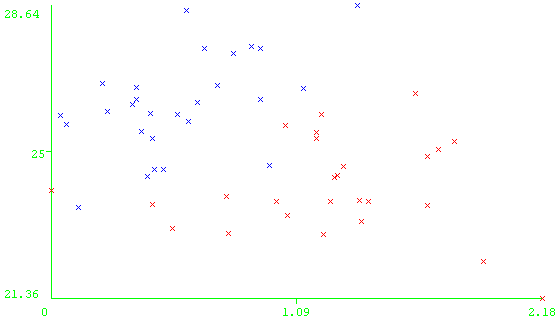
\includegraphics[scale=0.65]{cluster1.png}
    \end{centering}

    \textcolor{blue}{Cluster 0}: good courses --- \textcolor{red}{Cluster 1}: bad courses

\end{frame}

\begin{frame}{Cluster Analysis}{How can we evaluate the obtained clustering?}

\vspace{0.3cm}
\begin{centering}
    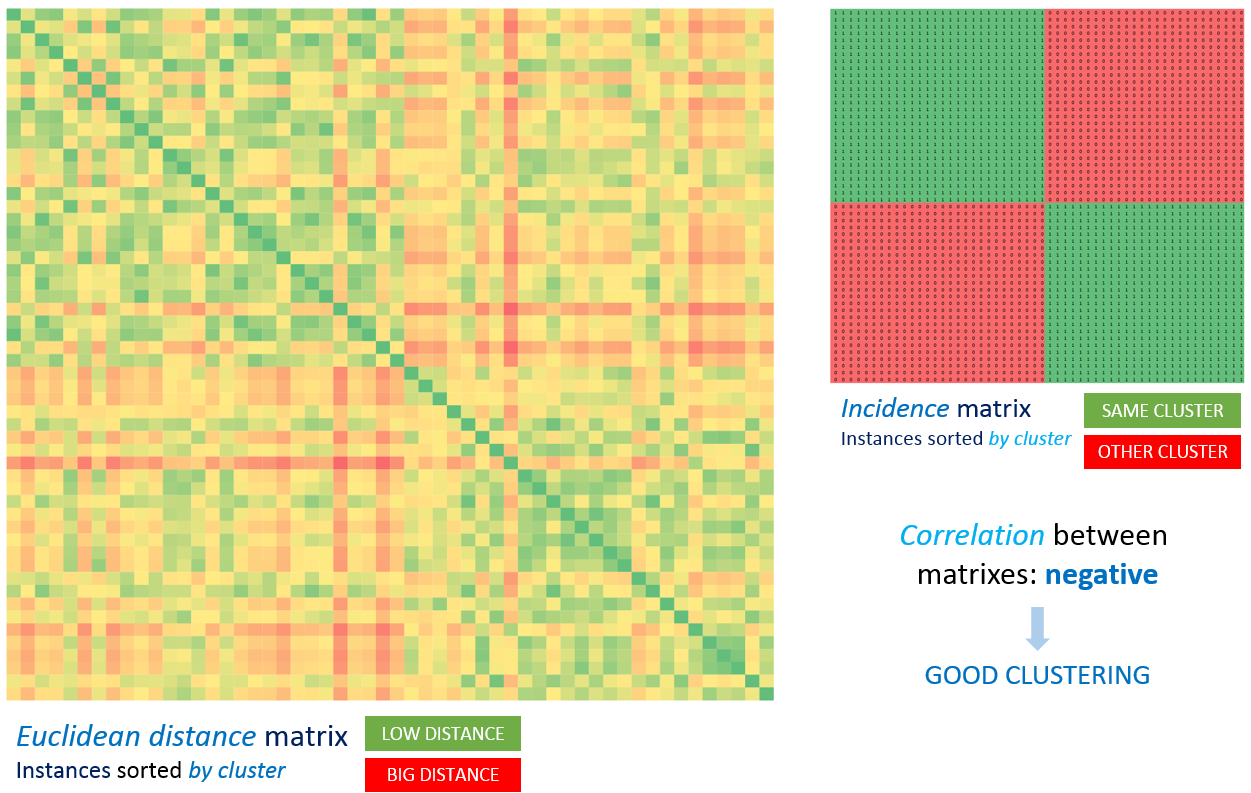
\includegraphics[scale=0.25]{cluster5_nocorr.png}
\end{centering}

\end{frame}

\begin{frame}{Cluster Analysis}{Cluster's composition: analysis and interpretation}

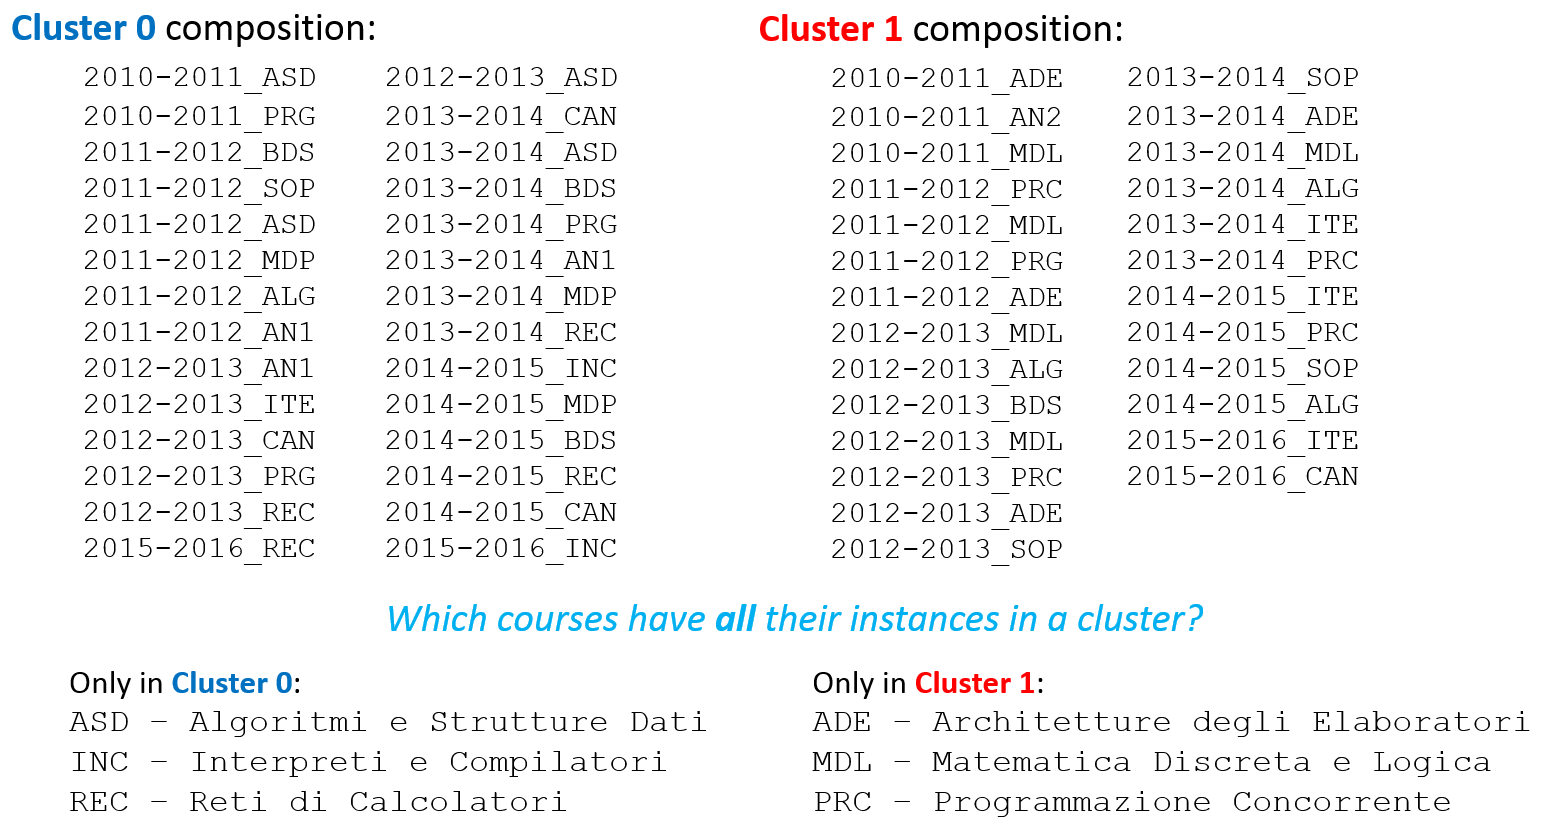
\includegraphics[scale=0.22, trim=2.2cm 0 0 0]{cluster6.png}

\end{frame}
